\section{Uran}
%jachymov, jak se objevil uran a ze je pojmenovanej podle planety uran
\subsection{Zpracování rudy}
%https://www.energy.gov/ne/fuel-cycle-technologies/uranium-management-and-policy/nuclear-fuel-cycle
\subsection{Možnosti obohacování}
\subsection{Způsoby měření obohacení}

\section{Fyzikální princip měření}
Celý princip spočívá v tom, že při dopadu gama fotonu na detektor, dojde k pohlcení a předání energie fotonu některému z \e , který pak buď předá svou energii na foton (scintilační detektory), nebo měříme jeho energii (polovodičové detektory), nebo převede tuto energii na energii chemickou.
\subsection{Druhy detektorů}
%objeveni gamma zareni
Henri Becquerel se v roce 1896 snažil přijít na to, jestli fosforujíci materialy nevydávají podobné záření jako nově objevené Rentgenové záření. Během čehož položil vzorek sulfidu uranu na fotocitlivý papír, který byl ještě zabalený, ale gamma zaření se podařilo proniknout skrz obal, na což přišel jakmile fotocitlivý papír vyvolal. Následně dělal mnoho dalších pokusů, aby potvrdil, že se nejedná o nějaký již známý efekt.  \cite{Radioactivity}%str 51
%TODO neelektricke detektory, historie

\subsubsection{Geigerův–Müllerův počítač}
Geigerův–Müllerův počítač funguje na principu, že když záření proniká vzduchem tak je schopno ionizovat molekuly vzduchu. Máme tedy 2 desky mezi kterými je vzduch, jakmile se vzduch ionizuje, díky velkému napětí na deskách dojde k lavinové ionizaci, která nám spoji obvod, což detekujeme na počitacím zařizení. Jsme tedy schopni určit kolik záření nám proniká, ale uz nejsme schopni říci o jaký druh záření se jedná, a natož o jakou energii.\\
Geigerův–Müllerův počítač je vhodný pouze v případech, kdy nepotřebujeme znát o jaký druh záření se jedná. Což je například když kontrolujeme zda je stínění dostatečné, chceme li se přesvědčit, zda je vzorek radioaktivní a také je hojně využíván v oblasti  jaderné bezpečnosti.\cite{}%TODO zdroj
\subsubsection{Scintilační detektory}
Scintilační detektory fungují na principu fluorescence a fosforescence, kde $\gamma$ foton excituje \e v atomu scintilacní látky, který když padá zpět z excitovaného stavu vyzáří foton viditelného světla, který následně zaznamenáváme.\cite{Knoll2010, Scintilators}
\subsubsection{Polovodičové detektory}
Polovodičový detektor je schopen merit energii s jakou foton dopada diky tomu ze pri fotoelektrickem jevu foton preda veskerou svou energii \e a ten pak dale vytrhava \e z el. obalu, diky cemuz jsme schopni urcit jakou energii foton mel. %TODO nejakou nevyhodu

\subsection{Principy měření gamma záření}%TODO udelat >>gamma<< jak promenou aby mi to nekde nekurvylo gama/ gamma kde bychn mel gamu v indexu!!
Gama záření s detektorem reaguje řadou fyzikálních dějů, mezi hlavní však patří fotoelktrický jev, Comptnův jev a tvorba párů \e a $e^+$. Pro tuto práci bude nejdůležitější fotoelktrický jev, protože se snažime určit energii relativně málo energetickým gama fotonů, které ani nejsou dostatečně silné aby dokázali vytvořit pár \e a $e^+$ \cite{DusanBc}
%TODO pridat obrazky k ruznym metodam
\subsubsection{Fotoelektrický effekt}
Když se do citlivé vrstvy detektoru (u germania díky speciální technice výroby velmi čistého germania v řádu \SI{}{\centi\meter}, u křemíku v řádu \SI{}{\milli\meter})  \cite{Knoll2010} %\footnote{G.F: Knoll str 415}
dostane $\gamma$ foton, tak díky fotoelektrickému jevu gama foton uvolní \e z elektronového obalu. Asi \SI{3}{\electronvolt} jsou potřeba na uvolnění \e z valenční vrstvy. (V případě Germania asi \SI{3,6}{\electronvolt}, v případě křemíku asi \SI{2,9}{\electronvolt}) \cite{astrnukleofyzika, nuclear_power-hpge}.\\ %\footnote{https://astronuklfyzika.cz/DetekceSpektrometrie.htm}
%\footnote{https://www.nuclear-power.com/nuclear-engineering/radiation-detection/semiconductor-detectors/high-purity-germanium-detectors-hpge/principle-of-operation-of-hpge-detectors}
Tato energie je nutná na odtržení \e od atomu. Zbylá energie gama fotonu se stane kinetickou energií \e. \uv{V polovodiči fotoelektron ztratí svou kinetickou energii při interakci elektromagnetickými silami s elektrony v polovodičové mřížce, čímž vzniká mnoho párů elektron-díra. Počet vytvořených párů elektron-děr je přímo úměrný energii dopadajícího fotonu.} \cite{semiconductors} %\footnote{Semiconductors for Room Temperature Nuclear Detector Applications, str. 23}%Albert Beer, Robert Willardson, Eicke Weber
Na diodu detektoru přivedeme v závěrném směru napětí, řadově tisíce~\SI{}{\volt} \cite{hpge-detector_fabrication}. %\footnote{https://sci-hub.se/10.1109/TNS.1972.4326520}
Jakmile se vytvoří pár \e~díra, tak se \e  přesouvá ke kladně nabité elektrodě, díra k záporně nabité, vzniká proud, a ten potom zaznamenáváme \cite{VUT,Knoll2010}. 
\subsubsection{Comptnův jev}
Prvním z nich je Comptonův jev, kde gama foton část své energie předá \e , který je vychýlen ze své původní dráhy. Foton změní směr pohybu a zvýší se jeho vlnová délka. \cite{robert_macku}
Tento foton může dále reagovat v detektoru, až dokud se nedostane mimo citlivou vrstvu detektoru, \break nebo dokud není zcela pohlcen.\\
\subsubsection{Tvorba párů \e a $e^+$}
Druhým z nich je tvorba páru elektron-pozitron, kdy pokud se $\gamma$ foton přiblíží k jádru atomu, tak se z jeho energie vytvoří pár \e, $e^+$. Musí se vytvořit oba, aby platil zákon zachování náboje. Jejich vytvoření neporušuje zákon zachování hmoty, protože platí teorie relativity, \break ze které vyplývá:  
\begin{equation}
	%https://opentextbc.ca/universityphysicsv3openstax/chapter/relativistic-energy/
	E^2 = (mc^2)^2 + (pc)^2
\end{equation}
Kde $E$ je energie fotonu, $m$ je hmotnost \e a $e^+$, kteří se vytvoří a $p$ je hybnost, která je rozdělena mezi ně a jádro atomu, u kterého se tato přeměna stane. 
Pokud měl foton větší energii než \SI{1022}{\kilo\electronvolt} \footnote{\SI{}{\electronvolt} je jednotka energie, je definována jako kinetická energie, kterou ve vakuu \e dostane  při urychlení napětím \SI{1}{\volt}. Energie komára je \SI{1e12}{\electronvolt}, jednotka je proto využívána v místech, kde jsou energie velmi malé, jako například v částicové fyzice.} \footnote{$m_{e} = \SI{9.1093837e-31}{\kilogram}$, $E=mc^2 \implies E = \SI{9.1093837e-31}{\kilogram} \cdot [\SI{299792458}{\meter\per\second}]^2 = \SI{8.1871058e-14}{\joule} =~\SI{510.999}{\kilo\electronvolt}$, je energie \e a protože vytváříme pár \e a $e^+$, potřebujeme 2 násobnou energii tj.~$\SI{1021.998}{\kilo\electronvolt}$}.\enlargethispage{\baselineskip} Pokud má $\gamma$ záření větší energii, tak tato energie je převedena na hybnost \e a $e^+$ \cite{semiconductors,libretext_pair}. %\footnote{ https://phys.libretexts.org/@go/page/10492} 
%\footnote{Semiconductors for Room Temperature, str. 23}
\section{Kalibrce HPGe detektoru}
Aby jsme byli schopni správně určit jakou mají energii neznámé vzorky musíme před tím určit jaké kanály přísluší jaké energii a jak je detektor na dané energie citlivý.
\subsection{Energetická kalibrace}%TODO OPRAVIT ty zarice jsem pouzil az na eff kalibraci
Při kalibraci jsem použil software GAMWIN, který je určený na~ovládání a~kalibraci gama detektorů. K změřeným kalibračním vzorkům (\ce{^{241}Am}, \ce{^{57}Co}, \ce{^{137}Cs}, \ce{^{133}Ba}, \ce{^{109}Cd}) jsem našel na \textit{Database WWW Table of Radioactive Isotopes}\footnote{\url{http://nucleardata.nuclear.lu.se/toi/nucSearch.asp}}
jejich energie gama rozpadu. Tyto energie jsem přiřadil k datům, která jsem naměřil, a následně jsem je proložil lineární funkcí. \cite{VUT} 
%TODO prepsat tak aby to odpovidalo

%TODO prvne jsem musel ty peaky najit pozil jsem prece ten program z reze
\subsection{Účinnostní kalibrace}
\begin{figure}[h!]
	\renewcommand\figurename{Graf}
	\centering
	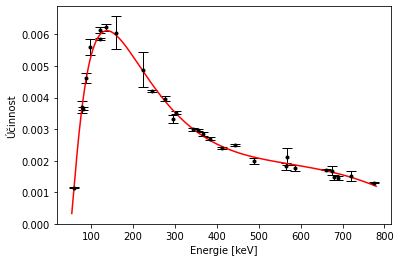
\includegraphics[width=0.7\linewidth]{eff_correct2.png}%TODO obrazek sem 80mm eff
	\caption{Závislost účinnosti na energii, pro pozici \SI{80}{\milli\metre} nad detektorem.}
	\label{fig:EFFvsENG5mm}
\end{figure}
Na výpočet efektivity detektoru, jsem použil rovnici  (\ref{eqn:effectivity}), která určí pro danou energii peakovou účinnost.
%První člen je zde pro počítaní efektivity.
%Druhý člen je na kompenzaci pro přeměnu mezi referenčním datem a datem měření. Třetí člen je zde pro kompenzaci přeměny během měření. %korekci/kompenzaci
\begin{equation}
	\label{eqn:effectivity}
	\varepsilon = \frac{S_{peaku}\lambda\frac{t_{real}}{t_{live}}}{A_0 I_\gamma}\cdot\frac{1}{e^{-\lambda t_0}}\cdot\frac{1}{1-e^{-\lambda t_{real}}}
\end{equation}
Kde $\varepsilon$ je peaková účinnost, $S_{peaku}$ je plocha peaku, bez plochy radiačního pozadí, $\lambda$ poločas přeměny  $t_{real}$ je doba, jak dlouho probíhalo celé měření, $t_{live}$ doba, jak dlouho detektor měřil (doba měření bez mrtvé doby detektoru), $A_0$ referenční aktivita kalibračního zdroje,  $I_\gamma$ je tabulková intenzita kalibračního zdroje a $t_0$ je doba mezi měřením a měřením referenční aktivity.
\subsection{Opravné faktory}
\subsubsection{Nelinearita}
\subsubsection{Samoabsorbce}
%TODO nekam napsat ze vzhlemed k vzdalenosti od detektoru muzeme nebodovost vzorku zanedbat
\section{Měření}
\subsection{Postup měření}%mozna to dat hned pod ten hlavni nadpis
\subsection{Výsledky měření} %TODO co jsem dát aniž by to nebyla tabulka na 3 strany
%TODO magic kterej je popsanej v vedeckejch studiich ktere jsem cetl
\newpage